\documentclass{beamer}
\usepackage[utf8]{inputenc}

\usetheme{Madrid}
\usecolortheme{default}
\usepackage{amsmath,amssymb,amsfonts,amsthm}
\usepackage{txfonts}
\usepackage{tkz-euclide}
\usepackage{listings}
\usepackage{adjustbox}
\usepackage[T1]{fontenc}
\usepackage{array}
\usepackage{tabularx}
\usepackage{gvv}
\usepackage{lmodern}
\usepackage{circuitikz}
\usepackage{tikz}
\usepackage{graphicx}

\setbeamertemplate{page number in head/foot}[totalframenumber]

\usepackage{tcolorbox}
\tcbuselibrary{minted,breakable,xparse,skins}



\definecolor{bg}{gray}{0.95}
\DeclareTCBListing{mintedbox}{O{}m!O{}}{%
  breakable=true,
  listing engine=minted,
  listing only,
  minted language=#2,
  minted style=default,
  minted options={%
    linenos,
    gobble=0,
    breaklines=true,
    breakafter=,,
    fontsize=\small,
    numbersep=8pt,
    #1},
  boxsep=0pt,
  left skip=0pt,
  right skip=0pt,
  left=25pt,
  right=0pt,
  top=3pt,
  bottom=3pt,
  arc=5pt,
  leftrule=0pt,
  rightrule=0pt,
  bottomrule=2pt,
  toprule=2pt,
  colback=bg,
  colframe=orange!70,
  enhanced,
  overlay={%
    \begin{tcbclipinterior}
    \fill[orange!20!white] (frame.south west) rectangle ([xshift=20pt]frame.north west);
    \end{tcbclipinterior}},
  #3,
}
\lstset{
    language=C,
    basicstyle=\ttfamily\small,
    keywordstyle=\color{blue},
    stringstyle=\color{orange},
    commentstyle=\color{green!60!black},
    numbers=left,
    numberstyle=\tiny\color{gray},
    breaklines=true,
    showstringspaces=false,
}
%------------------------------------------------------------
%This block of code defines the information to appear in the
%Title page
\title %optional
{ 5.3.12}

%\subtitle{A short story}

\author % (optional)
{Hemanth Reddy-AI25BTECH11018}



\begin{document}


\frame{\titlepage}
\begin{frame}{Question}
Solve for x and y\\

x + y = 6, 2x -3y = 4\\
\end{frame}



\begin{frame}{Theoretical Solution}
\textbf{Solution:}\\


Let :
\begin{align}
    \vec{r_1} = \myvec{1 & 1 }\vec{x} = 6 \\
    \vec{r_2} = \myvec{2 & -3}\vec{x} = 4
\end{align}

The augmented matrix of the above equations is given by,\\
\begin{align}
    \myvec{ 1&1&&6\\ 2&-3&&4} \stackrel{R_2 \leftarrow R_2 - 2R_1}{\longleftrightarrow}\myvec{ 1&1&&6\\ 0&-5&&-8} 
\end{align}

\begin{align}
    \myvec{ 1&1&&6\\ 0&-5&&-8} \stackrel{R_1 \leftarrow 5R_1 +R_2}{\longleftrightarrow}\myvec{ 5&0&&22\\ 0&-5&&-8} 
\end{align}


\end{frame}
\begin{frame}{Theoretical Solution}
\begin{align}
    5x=22 \qquad x=\frac{22}{5}\\
    -5y=-8 \qquad y=\frac{8}{5}
\end{align}
\end{frame}

\begin{frame}[fragile]
    \frametitle{C Code }
    \begin{lstlisting}

#include <stdio.h>

int main() {
    // Coefficients and constants for the system of linear equations
    // Equation 1: x + y = 6
    double a1 = 1.0;
    double b1 = 1.0;
    double c1 = 6.0;

    // Equation 2: 2x - 3y = 4
    double a2 = 2.0;
    double b2 = -3.0;
    double c2 = 4.0;

    // Use Cramer's Rule to solve for x and y
    // Determinant of the coefficient matrix
  


    \end{lstlisting}
\end{frame}

\begin{frame}[fragile]
    \frametitle{C Code }
    \begin{lstlisting}

  double determinant = a1 * b2 - a2 * b1;

    // Check if the determinant is close to zero, which means no unique solution exists
    if (determinant == 0) {
        printf("The system has no unique solution.\n");
        return 1;
    }

    // Determinant for x
    double determinant_x = c1 * b2 - c2 * b1;
    
    // Determinant for y
    double determinant_y = a1 * c2 - a2 * c1;



    \end{lstlisting}
\end{frame}




\begin{frame}[fragile]
    \frametitle{C Code }
    \begin{lstlisting}

    // Solve for x and y
    double x = determinant_x / determinant;
    double y = determinant_y / determinant;

    // Print the results
    printf("The solution to the system is:\n");
    printf("x = %.2f\n", x);
    printf("y = %.2f\n", y);

    return 0;
}

      \end{lstlisting}
\end{frame} 


\begin{frame}[fragile]
    \frametitle{Python Code }
    \begin{lstlisting}

import numpy as np
import matplotlib.pyplot as plt

def plot_solution():
    # Define the equations of the lines
    # Line 1: x + y = 6  =>  y = 6 - x
    # Line 2: 2x - 3y = 4  =>  y = (2x - 4) / 3

    # Generate x values to plot the lines
    x = np.linspace(-10, 10, 400)

    # Calculate corresponding y values for each line
    y1 = 6 - x
    y2 = (2 * x - 4) / 3

    # The solution is x = 22/5 = 4.4 and y = 8/5 = 1.6
    solution_x = 22 / 5
    solution_y = 8 / 5


      \end{lstlisting}
\end{frame} 

\begin{frame}[fragile]
    \frametitle{Python Code }
    \begin{lstlisting}


    # Set up the plot
    plt.figure(figsize=(8, 8))
    plt.title('Solution of the System of Linear Equations')
    plt.xlabel('x-axis')
    plt.ylabel('y-axis')
    plt.grid(True, linestyle='--', alpha=0.6)
    plt.axhline(0, color='black', linewidth=0.5)
    plt.axvline(0, color='black', linewidth=0.5)
    plt.axis('equal') # Ensures correct aspect ratio

    # Plot the lines
    plt.plot(x, y1, label='x + y = 6', color='blue')
    plt.plot(x, y2, label='2x - 3y = 4', color='red')

    

      \end{lstlisting}
\end{frame} 

\begin{frame}[fragile]
    \frametitle{Python Code }
    \begin{lstlisting}

# Plot and annotate the intersection point
    plt.plot(solution_x, solution_y, 'o', color='green', markersize=10, label=f'Solution ({solution_x:.1f}, {solution_y:.1f})')
    plt.annotate(f'({solution_x:.1f}, {solution_y:.1f})',
                 (solution_x, solution_y),
                 textcoords="offset points",
                 xytext=(0,10),
                 ha='center')

    # Add a legend and display the plot
    plt.legend()
    plt.show()

# Run the plotting function
plot_solution()

      \end{lstlisting}
\end{frame} 

\begin{frame}{Plot}

\begin{figure}
    \centering
    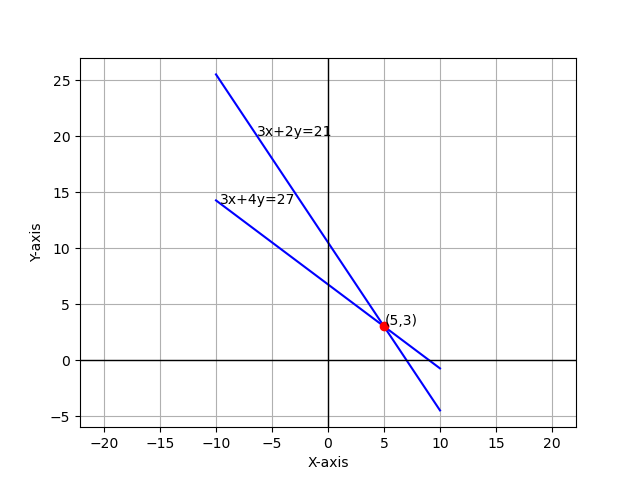
\includegraphics[width=0.6\linewidth]{Beamer/figs/plot.png}
    \caption{}
    \label{fig:placeholder}
\end{figure}

\end{frame}



\end{document}

